% vim:textwidth=70
\chapter{相关工作}
\label{chap:related}

本章介绍与本文内容相关的分布式系统管理与调试方面的研究工作。

% distributed platform

% 文件部署,自管理,self-*性质

% 承前启后:有什么什么工作,大致如何,有下面这些重要的工作
% 除了xxx,其它相关工作还有,它们有xxx特点、区别。


\section{分布式系统管理}

\ref{xxx}节首先叙述了一些常见的分布式应用管理系统,使读者对基本的管理系统
设计有所了解。数据分发是可自管理的分布式应用管理系统中的重点,\ref{xxx}节
介绍了一些重要的数据分发系统。

% 和自管理紧密相关的研究,epidemic algorithm,dissemination,self-*

% \subsection{management overview}
% 
% 从管理设计到的任务看:
% 
% *should not needed, duplicated in intro*
% 
% resource discovery: sword, xenosearch
% 
% dissemination: below
% 
% monitor: aggregation (pier, sophia, irisnet, mon, astrolabe, sdims,
% willow, SOMO, san femin, ganglia, )
% 
% and distributed trigger (sum -> complex operation -> topK -> quantiles
% -> set-expression, ok and enough)

\subsection{分布式应用管理系统}

分布式应用管理系统或工具对一个分布式计算平台来说是必不可少的。一些可以
公开或半公开访问的的分布式计算平台有
Planet-Lab~\cite{Bavier2004},TeraGrid~\cite{Catlett2002}和Amazon
EC2~\cite{Garfinkel2007}。在这些平台上,较多使用的管理工具有:

\subsubsection*{vxargs和pssh}

vxargs~\cite{vxargs}和pssh~\cite{pssh}是两个集中式管理工具,用一组脚本
实现。使用时,只需要将工具的脚本复制到发起管理的中心节点即可。它们利用
Unix/Linux平台安装的ssh/scp工具远程复制文件或执行控制命令。

\subsubsection*{Application Manager}

Application Manager~\cite{appmanager}(简称appmanager)也是一个集中管
理工具。它稍微复杂一点,有了自己的客户端。使用者首先将appmanager的客户
端安装到一组机器上并启动。客户端在运行时定期和服务器通信,询问有没有尚
未执行的用户命令。用户可以使用appmanager安装、查询与控制在客户端机器上
运行着的应用节点状态。

\subsubsection*{Plush}

Plush~\cite{plush}致力于提供一个全面的管理框架。它首先将管理
一个分布式应用的过程分为资源发现与获取、应用部署、应用维护三大部分。用
户使用XML语言描述应用管理涉及的这三部分内容,让Plush自动完成管理工作。

\begin{figure}
\centering
\begin{lstlisting}[language=XML,numbers=left]
<?xml_version="1.0" encoding="utf-8"?>
<plush>
    <project_name="sword">
        <software name="sword_software" type="tar">
            <package name="sword.tar" type="web">
                <path>http://plush.ucsd.edu/sword.tar</path>
                <dest>sword.tar</dest>
            </package>
        </software>
        <component name="sword_participants">
            <rspec>
                <num_hosts_min="10" max="800"/>
            </rspec>
            <resources>
                <resource_type="planetlab" group="ucsd_sword"/>
            </resources>
            <software_name="sword_software"/>
        </component>
        <application_block name="sword_app_block" service="1"
            reconnect_interval="300">
            <execution>
                <component_block_name="participants">
                    <component_name="sword_participants"/>
                    <process_block name="sword">
                        <process name="sword_run">
                            <path>dd/planetlab/run sword</path>
                        </process>
                    </process_block>
                </component_block>
            </execution>
        </application_block>
    </project>
<plush>
\end{lstlisting}
\caption{Plush应用管理说明}
\label{fig:plush_spec}
\end{figure}


图~\ref{fig:plush_spec}是用Plush管理SWORD~\cite{sword_worlds,
sword_toit}的XML说明。在\texttt{software}标签里,指明了SWORD的安装程序
地址是\texttt{\url{http://plush.ucsd.edu/sword.tar}}。在
\texttt{component}标签,指明了运行SWORD需要Planet-Lab上至少10个,至多
800个机器,但是没有指明机器的属性。在\texttt{application\_block}标签,
指明了应用执行与维护相关的参数,例如SWORD的执行路径是
\texttt{dd\-/planetlab\-/run sword},SWORD的维护策略是\texttt{service
(service="1")}等等。

Plush也采用了集中式管理的策略,有自己的客户端,通过客户端与服务器端的
通信完成管理任务。Plush具备一定的自管理能力。在运行时,如果发现某个机
器上没有运行Plush客户端,服务器端会自动将Plush客户端安装至远程机器。然
而这个过程也是使用集中式算法实现,因而可扩展性不好,也不能应对网络分割
问题。

Plush-M~\cite{plush-m}注意到了Plush采用集中式算法的问题。它将Plush中服
务器到客户端之间的星型拓扑,替换为RanSub~\cite{ransub}组播树。提高了系
统的可扩展性,与应对网络分割错误的能力。需要注意到,这仅仅改变了Plush
管理其它应用的方式,并没有改变Plush自管理的方式。

\subsubsection*{Globus}

Globus~\cite{globus}是搭建Grid系统与应用的软件工具包。它包含了应用管理
的组件。例如,可以使用Globus Resource Specification Language (RSL)描述
对资源的需求,使用Globus Resource Allocation Manager (GRAM)为应用分配
资源。


% Amazon EC2怎么怎么(就不用开个小标题了)

% smartfrog cfengine

\subsection{数据分发}

\subsubsection*{BitTorrent}

BitTorrent~\cite{bittorrent}是一个Peer-to-Peer(P2P)文件共享协议,它是
Internet上使用最广泛的文件分发、共享工具。一些估算表明,它产生的网络通
信占整个Internet流量的35\%~\cite{bt2004}。

Bittorrent由一组节点(peer)和一个tracker构成。初始时,有一个节点包含
了整个要共享的文件,它被称为种子。其它节点可以从种子下载文件。同时,节
点还可以通过tracker获取其它节点的列表,并相互交换没有的文件块。这样,
不仅加速了文件共享传输的速度,也减轻了种子节点的带宽消耗。

由于Bittorrent出色的性能,它也被用来在Planet-Lab平台上部署
分发数据~\cite{plDist}。

\subsubsection*{ACMS}

Akamai~\cite{akamai}是运营着一个全球范围的内容分发网络(Content
Distribution Network, CDN),包括了部署在60多个国家的1200多个ISP的超过
15000个服务器。用户可以使用Akamai分发自己的网络内容与服务,提高应用的
性能和可靠性。

ACMS~\cite{acms}(The Akamai Configuration Management System)是Akamai的
配置管理工具。它将用户对分发内容的配置部署到CDN网络内。这面临着很多挑
战。使用ACMS的用户来自世界各地,可以在任何时间访问系统。首先需要保证服
务可用性。ACMS使用了多个服务入口点(entry point)接受配置文件更新的请
求,入口点分布在不同的ISP内。其次,同一配置,可能会被不同的人同时更新,
更新请求可能会同时到达不同的入口点。需要保证更新的一致性。ACMS使用了基
于向量交换(Vector Exchange)的quorum算法,让入口点之间对更
新顺序达成一致意见,保证了更新的正确性。

\begin{figure}
\centering
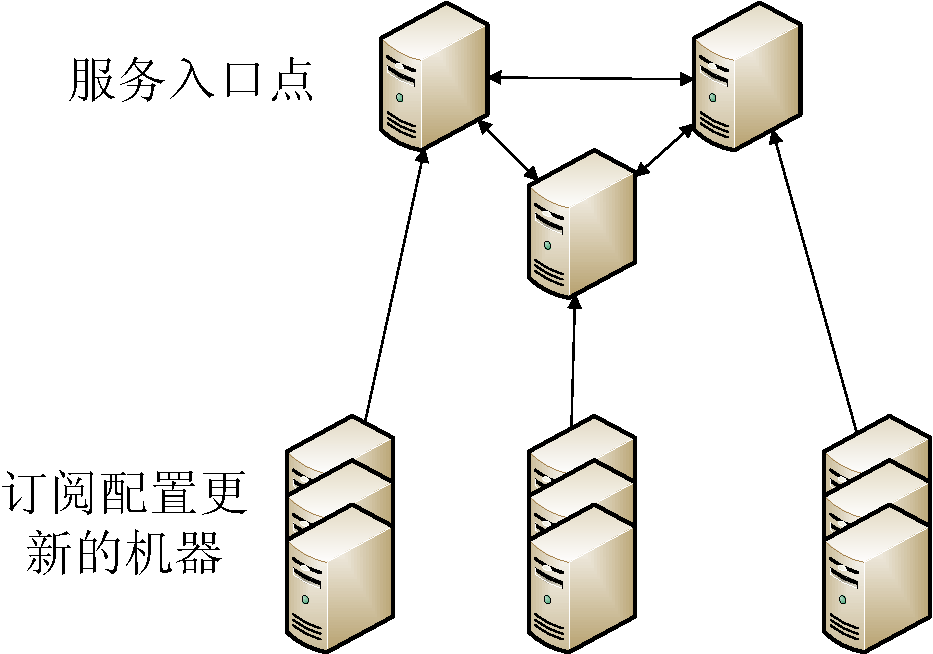
\includegraphics[width=0.8\linewidth]{acms_design}
\caption{ACMS系统结构}
\label{fig:acms_design}
\end{figure}


为了同时保证更新能够快速有效的被传送到整个CDN的所有机器上,ACMS将更新
分为两部进行,如图~\ref{fig:acms_design}所示。更新首先由用户发送到某
一个入口点,这个入口点服务器和其它服务器达成对更新的一致意见后,将更新
持久化保存到各自的硬盘上,并给用户返回更新成功。其它CDN的节点会定期向
入口点查询订阅的配置文件的版本,并从入口点机器下载更新。通过利用CDN节
点的HTTP缓存机制,更新可以快速的被传递到所有的CDN机器上。

ACMS使用的分层部署方法将更新的正确性和性能问题分开解决。入口点机器通过
使用quorum算法解决了正确性问题,其它节点向入口点机器订阅更新,解决了更
新传递的性能问题。

\subsubsection*{CoDeploy}

CoDeploy~\cite{codeploy}利用了CoDeeN~\cite{codeen}内容分发网络帮助人们
在Planet-Lab平台上部署应用与数据。由于部署的内容可能很大,而CoDeeN使用
了基于HTTP缓存的内容分发技术,因此CoDeploy首先将要部署的内容打成碎片。
在部署的目标节点上分别下载各个碎片后,再将原来的部署数据复原。

\subsubsection*{SharkFS}

SharkFS~\cite{sharkfs}使用了合作缓存(Cooperative Caching)技术提高了
网络文件系统的可扩展性。通常在网络文件系统中,客户端会向文件系统服务器
所要数据,服务器会成为性能瓶颈。SharkFS让客户端之间相互下载自己没有对
方有的文件块来解决这个问题。这个方式类似于Bittorrent。与Bittorrent不同
的是,SharkFS中没有集中的tracker,而是让所有客户端之间形成一个结构化覆
盖网络\cite{can, pastry, tapestry, chord, kademlia},实现了一个分布式
的tracker。

\subsection{self-*}

自稳\cite{Dijkstra1974}(self-stablization)是一个分布式系统中的容错概
念,在1974年由E.\ W.\ Dijkstra提出。它是指,系统从任何状态开始,都会自动
收敛于合法的状态。这是一个很强的属性。由于分布式系统难于调试与分析,因
此这个属性是很受期待的。

IBM在2001年提出了Automatic Computing~\cite{Kephart2003}(AC)的概念。
由于分布式系统越来越大,其管理复杂度也越来越高。AC旨在让分布式系统具备
自我管理的能力,能够自动应对各种不可预期的错误。在AC中,系统行为用闭环
控制(closed control loops)建模,从而能够自动监测外部状态改变,并自动
调整自己的行为。

DHT~\cite{can, pastry, tapestry, chord, kademlia}(Distributed Hash
Table)能够自动应对系统的节点加入与退出事件,通过调整每个对等节点的路
由表,自动维护设计的拓扑结构。\note{自动维护replica}

Rhizoma~\cite{Rhizoma}试图将自我管理功能嵌入到分布式应用内部去。它的研
究动机是,随着Utility Computing(UC)的出现,将有越来越多的公司将自身
的计算需求外包给计算服务提供商,例如Amazon EC2~\cite{Garfinkel2007}。
运行在UC计算平台的应用有依据资源使用状况、节点失败和计费等情况迁移到其
它节点的需求。这个问题可以利用管理工具实现,Rhizoma试图将自我管理功能
内嵌到应用来解决这个问题。

% SCAMP self-organizing membership

\section{分布式系统调试}

First, execution of a transaction is often distributed across process
and machine boundaries. Second, an executing stage may be a process, a
thread, an event, or a stage worker thread (as in the Staged Event
Driven Architecture (SEDA) [25]). A transaction needs to be tracked
across all such stages. Third, threads may pass a particular
transaction between them- selves via shared memory. Shared memory
communications are generally harder to track than inter-process
communication (IPC) via the operating system or middleware. Finally,
due to concurrent execution, a transaction may cause another
transaction to wait, e.g., due to lock contention.


分布式系统调试的难点在于任务会被分为不同的部分或阶段,分散在系统的不同
机器、进程和线程执行。错误:执行顺序,状态变化

topic: task model/execution path reconstruction, inference, graph
mining

我们使用图上的聚类算法研究了自动推断任务模型的方法,涉及到xxx个主题,
任务模型,图聚类,分别叙述相关工作如下。

log mining related

\subsection{task model control flow}

*white box*

获取系统对每个请求的执行路径,也就是请求在系统中被处理的过程,是分析系
统行为,找到错误根本原因的一个基本方法。

(pinpoint) The path abstraction has been used in many other areas,
typically as a form of control flow. Paths are used in Scout for a
single-node OS [38], are the foundation for
integrated-layer-processing [1], and play a key role in many compiler
optimization techniques [5]. Several recent systems have also used
paths to profile distributed systems.

路径:控制路径,数据路径


执行路径也可以被称为因果路径(causal path),因为

% Performance Debugging for Distributed Systems of Black Boxes
% (sosp03)

\subsubsection*{Pinpoint}

% see related in reynolds thesis

Pinpoint~\cite{pinpoint}通过对系统增加标注的办法,为J2EE应用的每个用户
请求附加了一个唯一标识。标注就是对系统代码进行一定修改,在适当的地方输
出与传递任务标识。随着请求被处理,和它关联的标识也在系统中传播,从而我
们可以追踪得到每个请求在系统中处理的执行路径。

进一步的,Pinpoint可以找到执行路径中的异常。所谓异常并不一定是系统的软
件错误。Pinpoint的假设是,系统错误是较少发生的,因此那些有异常的执行路
径可能代表系统错误的发生。这一方法对多数情况是有效地,但是也会造成一些
漏判,也就是把一些的确有错误的执行路径当成正常情况。

Pinpoint使用概率上下文无关文法(Probabilistic Context Free
Grammar,PCFG~\cite{Manning1999},来检测有异常的执行路径。也就是,
Pinpoint记录了执行路径上的事件会以什么概率导致其它事件发生。例如,一个
事件$A$发生后,可能会接着发生事件$B$或$C$。所以,如果观测到$A \to D$,
则这是一个异常事件。

\subsubsection*{Magpie}

与Pinpoint不同,Magpie~\cite{magpie}并不对每个请求增加标注,而是使用用
户提供的方案(schema)将观测到的系统事件联系成为任务执行路径。Magpie将
得到的执行路径用聚类算法分类,每一类称为一个负载模型,描述了某一种请求
在系统中处理的典型路径和资源消耗情况。使用负载模型,可以对系统性能进行
分析与预测。

Magpie基于Windows平台。它使用ETW(Event Tracing for
Windows)~\cite{etw, Park2003}机制收集系统执行过程中发生的事件。ETW是
Windows平台内建的消息追踪机制,追踪与输出事件的额外负载(overhead)很
低。Windows操作系统在运行时就输出很多预设的ETW事件,这些事件可以作为
Magpie的输入。为了得到系统运行时的内部事件,可以使用插装的方法动态输出
系统内部状态。插装并不改变系统代码。ETW事件中包含了关于系统资源(CPU,
内存等)使用情况的信息,因而可以明确得到请求执行过程中消耗资源的详细信
息。

Magpie设计的特别之处在于使用用户提供的方案将属于同一请求的事件联合
(join)到一起,联合操作的语意借用了数据库的思想。详细描述如何编写方案
、不同的事件是如何被联合到一起超出本文的范围。简单举例说,如果一组事件
的ThreadID属性(表示事件在哪个线程发生)相同,则这组事件可以用ThreadID
联合到一起。考虑到资源复用的情况,例如线程池内的不同线程会在不同的时间
段处理不同的请求,Magpie借用了时间联合~\cite{Gao2005}(temporal join)
的思想,方案中同时描述了被联合属性的有效时间区间,从而,线程处理不同请
求的时间段可以被区分开,其它类似情况也可以被处理。

正确的编写方案要求用户对系统有深入的理解。用户需要正确的写出事件如何联
合起来,定义联合属性的有效时间区间,需要用户是专家级人员,例如系统的设
计与开发者。

\subsubsection*{pip}

Pip~\cite{pip}对代码增加标注,得到系统的执行路径。Pip定义了一个声明式
期望语言(declarative expectation language)。使用期望,用户可以表达系
统的运行时行为应该是什么样子的,通过将期望与实际运行获得的执行路径进行
对比,用户可以发现可能的系统错误,并使用运行时执行路径帮助找到错误发生
的原因。由于执行路径中包含了结构、时间和资源消耗的信息,Pip可以有效的
同时检查系统正确性错误与性能错误。

pip的期望示例。

\subsubsection*{X-Trace}

X-Trace~\cite{x-trace}是一个网络层的跟踪工具。它将包括任务标示符的任务
元数据嵌入用户请求(例如一个web请求)中,随着用户请求在网络上被向前传
送与处理,我们就能够得到这个请求在网络上处理的整个过程。任务元数据不仅
在同一层次的网络协议中传播,同时也被推送到下层协议中(例如从TCP到IP)。
这样,一个请求在网上被处理的过程就形成了一个完成的任务树。这能够帮助我
们理解请求在网络协议层次的因果路径。

图xxx显示了一个HTTP请求通过一个代理被发送到HTTP服务器的因果路径。

对于一些网络协议,X-Trace可以在消息包头的扩展域内添加任务元数据,这些
元数据会在处理的过程中自动传播,例如HTTP,SIP,Email和IP协议。TCP协议
虽然支持嵌入扩展信息,但是只支持一跳传播,需要改变Linux内核让元数据自
动传播到下一条去。对于一些复杂的应用层协议,例如Chord~\cite{chord},由
于Chord节点会对消息进行一些复杂处理,才生成新的路由消息,需要对Chord代
码进行一些更改才能支持元数据自动传播。

\subsection{inference}

上面这些工作把系统当作白盒,也就是认为我们可以得到系统内部的状态信息,
或者我们能够通过标注或者插装的方法改变系统行为。这个假设并不一定总能满
足。在系统中通常会使用第三方软件,例如在Web服务中后端的数据库系统。这
些系统可能是商业软件,因此不提供代码。这时基于白盒假设的调试工具就会失
去作用。

针对这个问题,一些基于黑盒假设的分析与调试工具被提出,以Project
5~\cite{project5},WAP5~\cite{wap5},sherlock~\cite{sherlock}为代表。
这些工具分析系统组件之间的消息通信,推断出请求被处理的因果路径。并分析
在消息处理层次,系统性能的瓶颈所在。

由于不能得到确切的系统状态,因此这些工具的推断结果只是概率意义上的,并
不完全准确。这些工具即使是对白盒系统也是有意义的。因为理解系统内部工作
机制,对系统增加标注并不容易,需要花费很长时间。基于黑盒假设的工具可以
很快的给出系统运行的大概情况,帮助人们尽快理解系统。

\subsection{dataflow}

请求被处理的执行路径,或者因果路径表示了请求处理的控制流信息。还有一些
工作通过获取系统运行时的数据流信息,分析系统行为。包括
Whodunit~\cite{whodunit} 和Data Flow Tomography~\cite{dft}等。

\subsubsection*{Whodunit}

Whodunit~\cite{whodunit}提出了事务概要分析(transactional profiling)
的概念和方法,这是对调用图概要分析(call graph
profiling)~\cite{Graham2004}和调用路径概要分析(call path profiling)~
\cite{Hall1992, Hall1993}的一个扩展。所谓事务并不是数据库中事务的概念,
而是表示分布式系统对外来的用户请求处理的整个过程。

Whodunit将事务的执行过程分为若干阶段(stage),每个阶段都可能在不同的
机器、进程和线程执行。阶段之间通过一定的数据共享或传输方式进行交互。
Whodunit考虑了三种数据共享或传输的方式,共享内存,事件和网络消息传递。

Whodunit通过分析线程之间的数据流扑捉事务通过共享内存传递的过程,
Whodunit借助虚拟机~\cite{qemu}截取所有的内存操作汇编指令做到这一点。这
个方法能够获取细粒度的事物传递过程,同时也不用修改系统代码。但是由于使
用了虚拟机,因而带来比较大的额外负载。

对于事物通过事件传递的情况,Whodunit需要在事件中添加事物信息。随着事件
在不同的阶段传递,就能得到事物处理的过程。这需要对事件处理的中间件
~\cite{seda}插装才能做到。类似的,Whodunit需要在网络消息中添加事物信息,
才能追踪事物通过网络传递的情况,它通过对\texttt{send}和
\texttt{receive}函数包装,并让应用调用包装后的\texttt{send}和
\texttt{receive}函数做到这一点。

\subsubsection*{Data Flow Tomography}

Data Flow Tomography~\cite{dft}的想法受到正电子发射断层扫描(Positron
Emission Tomography)的启发。正电子发射断层扫描技术将存活期短的放射性
同位素注入人体,通过观测它在人体内流动的过程,能够对病况进行诊断。

类似的,Data Flow Tomography工作对数据添加标记,从而可以观测到数据是如
何在系统中被处理和传递的整个过程。这包括,数据通过函数参数在不同的函数
抽象层传播,数据通过共享内存在线程间传播,数据通过网络传播等等情况。这
样,就能够回答诸如某个数据会产生哪些数据,某个数据由哪些数据生成等等问
题。

Data Flow Tomography通过使用虚拟机~\cite{qemu}追踪指令级(ISA)的数据
处理过程。这个做法的好处是不需要对应用做任何修改,但是反面作用是分析的
额外负载会很大。

% \subsection{graph mining} briefly

\subsection{log mining}

% see log-mining paper (wasl \& sysml)

系统日志是系统运行过程中产生的、对系统运行活动的描述,包含了很多应用层
任务流的语意,它是理解系统运行,调试系统问题的重要资源。

\subsubsection*{SALSA}

SALSA~\cite{salsa}在Hadoop~\cite{hadoop}日志上,提取出分布式系统的控制
流和数据流,并导出系统在每个节点上的状态机形式的运行过程。利用产生的结
果,SALSA可以对系统失败原因进行检查,并将系统的分布式行为可视化。

\subsubsection*{CLUEBOX}

CLUEBOX~\cite{cluebox}使用了机器学习方法,对系统的性能日志进行分析,提
取出系统的负载-性能模型。对于性能问题,CLUEBOX能够很快的将问题定位于相
关的一组性能计数器(performance counter)。

\subsubsection*{Artemis}

Artemis~\cite{artemis}是一个日志分析框架,包含了日志收集、日志存储、可
视化工具和一组插件定义接口,使用它,用户可以自定义插件,对系统(例如
Dryad~\cite{dryad})进行分析。

\section{本章小结}

本章对xxx进行了介绍,虽然xxx,但是xxx问题仍然是xxx面临的挑战。
